\section{Matlab program med alle amplitude- og fase-plot}\label{sec:spm5}

Ved gennemgang af måledata viser det sig, at der ved optagelse af ESR i figur \ref{fig:esrplot} er en faktor 10 til forskel fra at den korrigerede model passer bedre overens med det målte resultat.
Dette skyldes sandsynligvis med fejlindstilling i Bode100. 
Således bliver $r = 0,254 \si{\ohm}$ brugt i den korrigerede model som ses i figur \ref{fig:bodeplot_all}. 

\begin{figure}[h!]
	\centering
	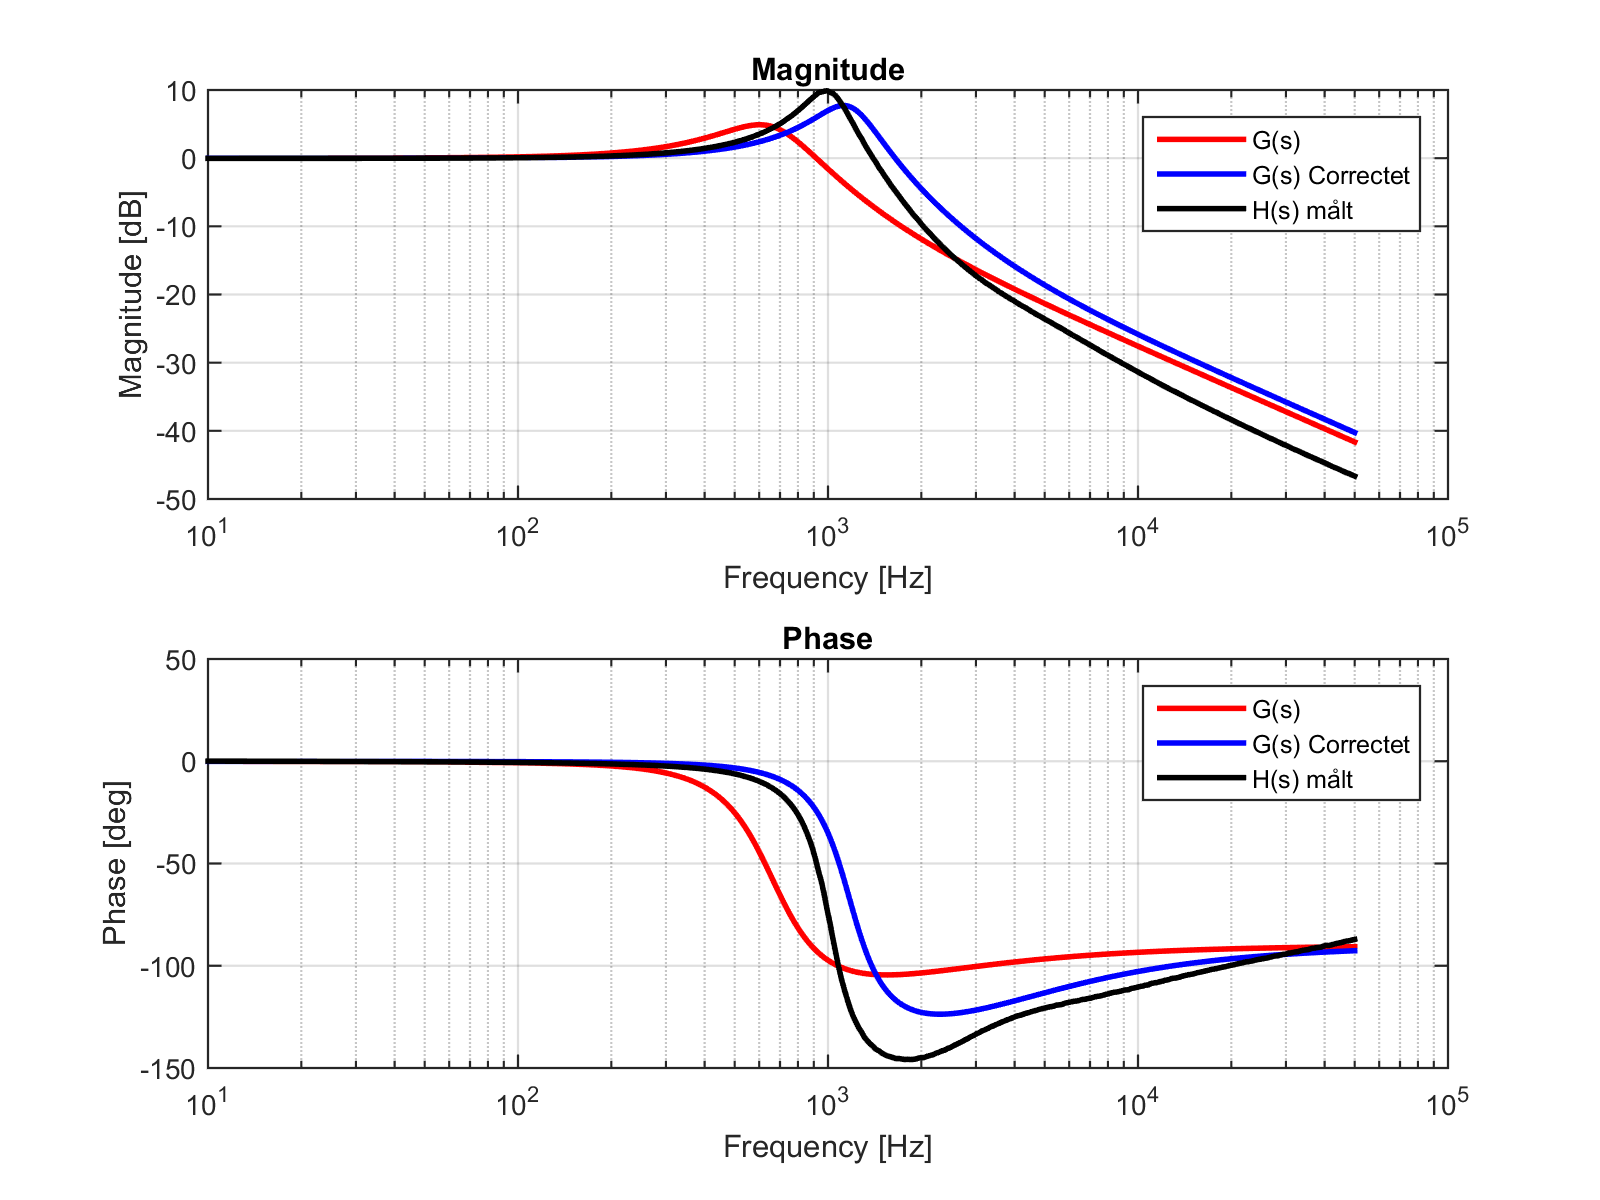
\includegraphics[width=.8\textwidth]{bodeplot_all.png}
	\caption{Bodeplot fra Matlab af Model (rød), Korrigeret Model (blå) og målt overførelsesfunktion (sort).}
	\label{fig:bodeplot_all}
\end{figure}
\FloatBlock

Matlab koden til fremstilling af figur \ref{fig:bodeplot_all} ses i appendiks \ref{bilag:reg1_all.m}